\begin{frame}{Online OWL reasoning-based approach}

    An approach focusing on OWL.
    
    \begin{itemize}
        \item An Information Retrieval ontology.
        \item Push knowledge closer to the data.
        \item Model domain knowledge as linked sets of taxonomies. 
    \end{itemize}

    Competency questions:
    \begin{itemize}
        \item CQ1 What are the categories in the user search?
        \item CQ2 What are the documents relevant to a search?
        \item CQ3 What categories are enabled to refine the search?
    \end{itemize}

\end{frame}

\begin{frame}{Information Retrieval Ontology}

    7 classes:
    \begin{itemize}
        \item \emph{CandidateDocument} subclass of \emph{Document} 
        \item \emph{SelectedCategory} and \emph{EnabledCategory} subclasses of \emph{Category}
        \item \emph{SearchContext} subclass of \emph{Search}
    \end{itemize}

    6 object properties:
    \begin{itemize}
        \item \emph{categorises} inverse of \emph{categorisedBy}
        \item \emph{hasSearchCategory} subproperty of \emph{enablesCategory}
        \item \emph{hasDirectSubcategory} subproperty of \emph{hasSubcategory}
    \end{itemize}

\end{frame}

\begin{frame}{Pizza ontology}

    Pizza ontology:
    \begin{itemize}
        \item Due to time constraints, we use the Pizza ontology for our demonstration.
        \item Well-known ontology built to introduce RDF/RDFS/OWL with examples (and even SHACL)
        \item Simple ontology with class hierarchies of:
        \begin{itemize}
            \item \emph{Pizza} (\emph{hasTopping}, \emph{hasBase})
            \item \emph{PizzaBase}
            \item \emph{PizzaTopping}
        \end{itemize} 
    \end{itemize}

\end{frame}

\begin{frame}{Pizza ontology KG-based IR system}

        \begin{center}
            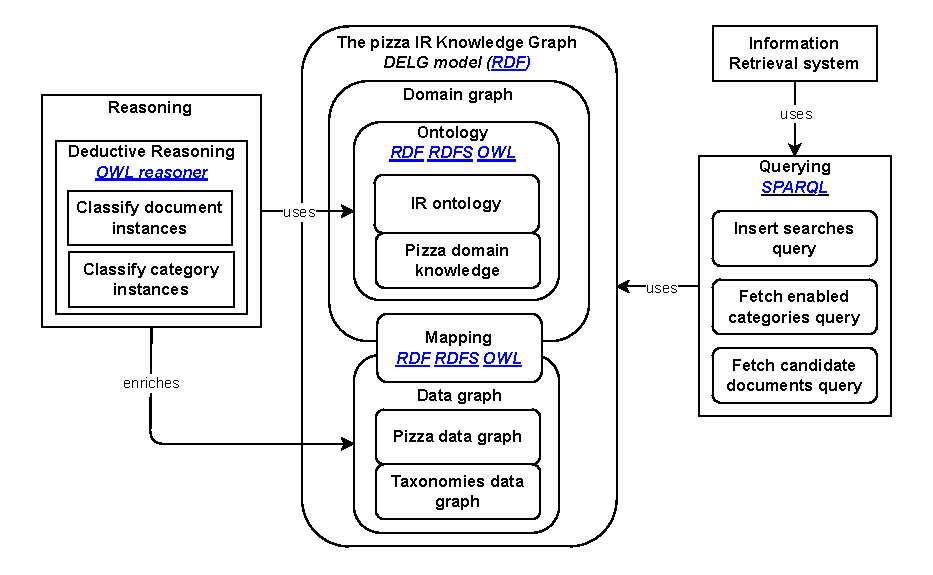
\includegraphics[scale=0.65]{images/pizza-demo-kg.pdf} 
        \end{center}

\end{frame}

\begin{frame}{Advantages and limitations}

    Advantages:
    \begin{itemize}
        \item Explicitly defines the notions of documents and categories
        \item New taxonomies can easily be integrated
    \end{itemize}

    Limitations:
    \begin{itemize}
        \item Requires one ontology instance per user query (Scaling limitation)
        \item Restricting search by conjunction of categories is a challenge (OWA limitations)
        \item Assumes an ontology structured as a set of interlinked taxonomies
    \end{itemize}

\end{frame}